\documentclass[border=6pt]{standalone}
\usepackage{fontspec}
\setmainfont{lmroman10-regular.otf}[BoldFont=lmroman10-bold.otf, ItalicFont=lmroman10-italic.otf, BoldItalicFont=lmroman10-bolditalic.otf]
\setmonofont{lmmono10-regular.otf}[BoldFont=lmmonolt10-bold.otf, ItalicFont=lmmono10-italic.otf]
\usepackage{tikz}
\usetikzlibrary{arrows.meta,positioning,fit,calc,backgrounds}

% The README's figure. Build: xelatex level1-flow.tex, then pdftoppm -png -r 200 -singlefile level1-flow.pdf level1-flow
% the colours of the proof pipeline's Figure 3
\definecolor{agentfill}{RGB}{238,237,253}
\definecolor{agentdraw}{RGB}{90,82,181}
\definecolor{agenttext}{RGB}{43,39,104}
\definecolor{measfill}{RGB}{229,244,238}
\definecolor{measdraw}{RGB}{62,122,101}
\definecolor{meastext}{RGB}{24,64,50}
\definecolor{fixedfill}{RGB}{241,239,233}
\definecolor{fixeddraw}{RGB}{138,136,131}
\definecolor{fixedtext}{RGB}{51,51,51}
\definecolor{arrowc}{RGB}{112,112,112}

\tikzset{
  box/.style={rounded corners=2pt, line width=0.6pt, align=center, inner sep=5pt, font=\small},
  agent/.style={box, draw=agentdraw, fill=agentfill, text=agenttext},
  meas/.style={box, draw=measdraw, fill=measfill, text=meastext},
  fixed/.style={box, draw=fixeddraw, fill=fixedfill, text=fixedtext},
  opt/.style={dash pattern=on 3pt off 2pt},
  arr/.style={-{Stealth[length=2.2mm,width=1.6mm]}, draw=arrowc, line width=0.6pt},
  lab/.style={font=\small, text=fixedtext, align=left},
}
\newcommand{\tit}[1]{{\normalsize\bfseries #1}\\[1pt]}
\newcommand{\tool}[1]{{\normalsize\ttfamily\bfseries #1}\\[2pt]}

\begin{document}
\hyphenpenalty=10000 \exhyphenpenalty=10000
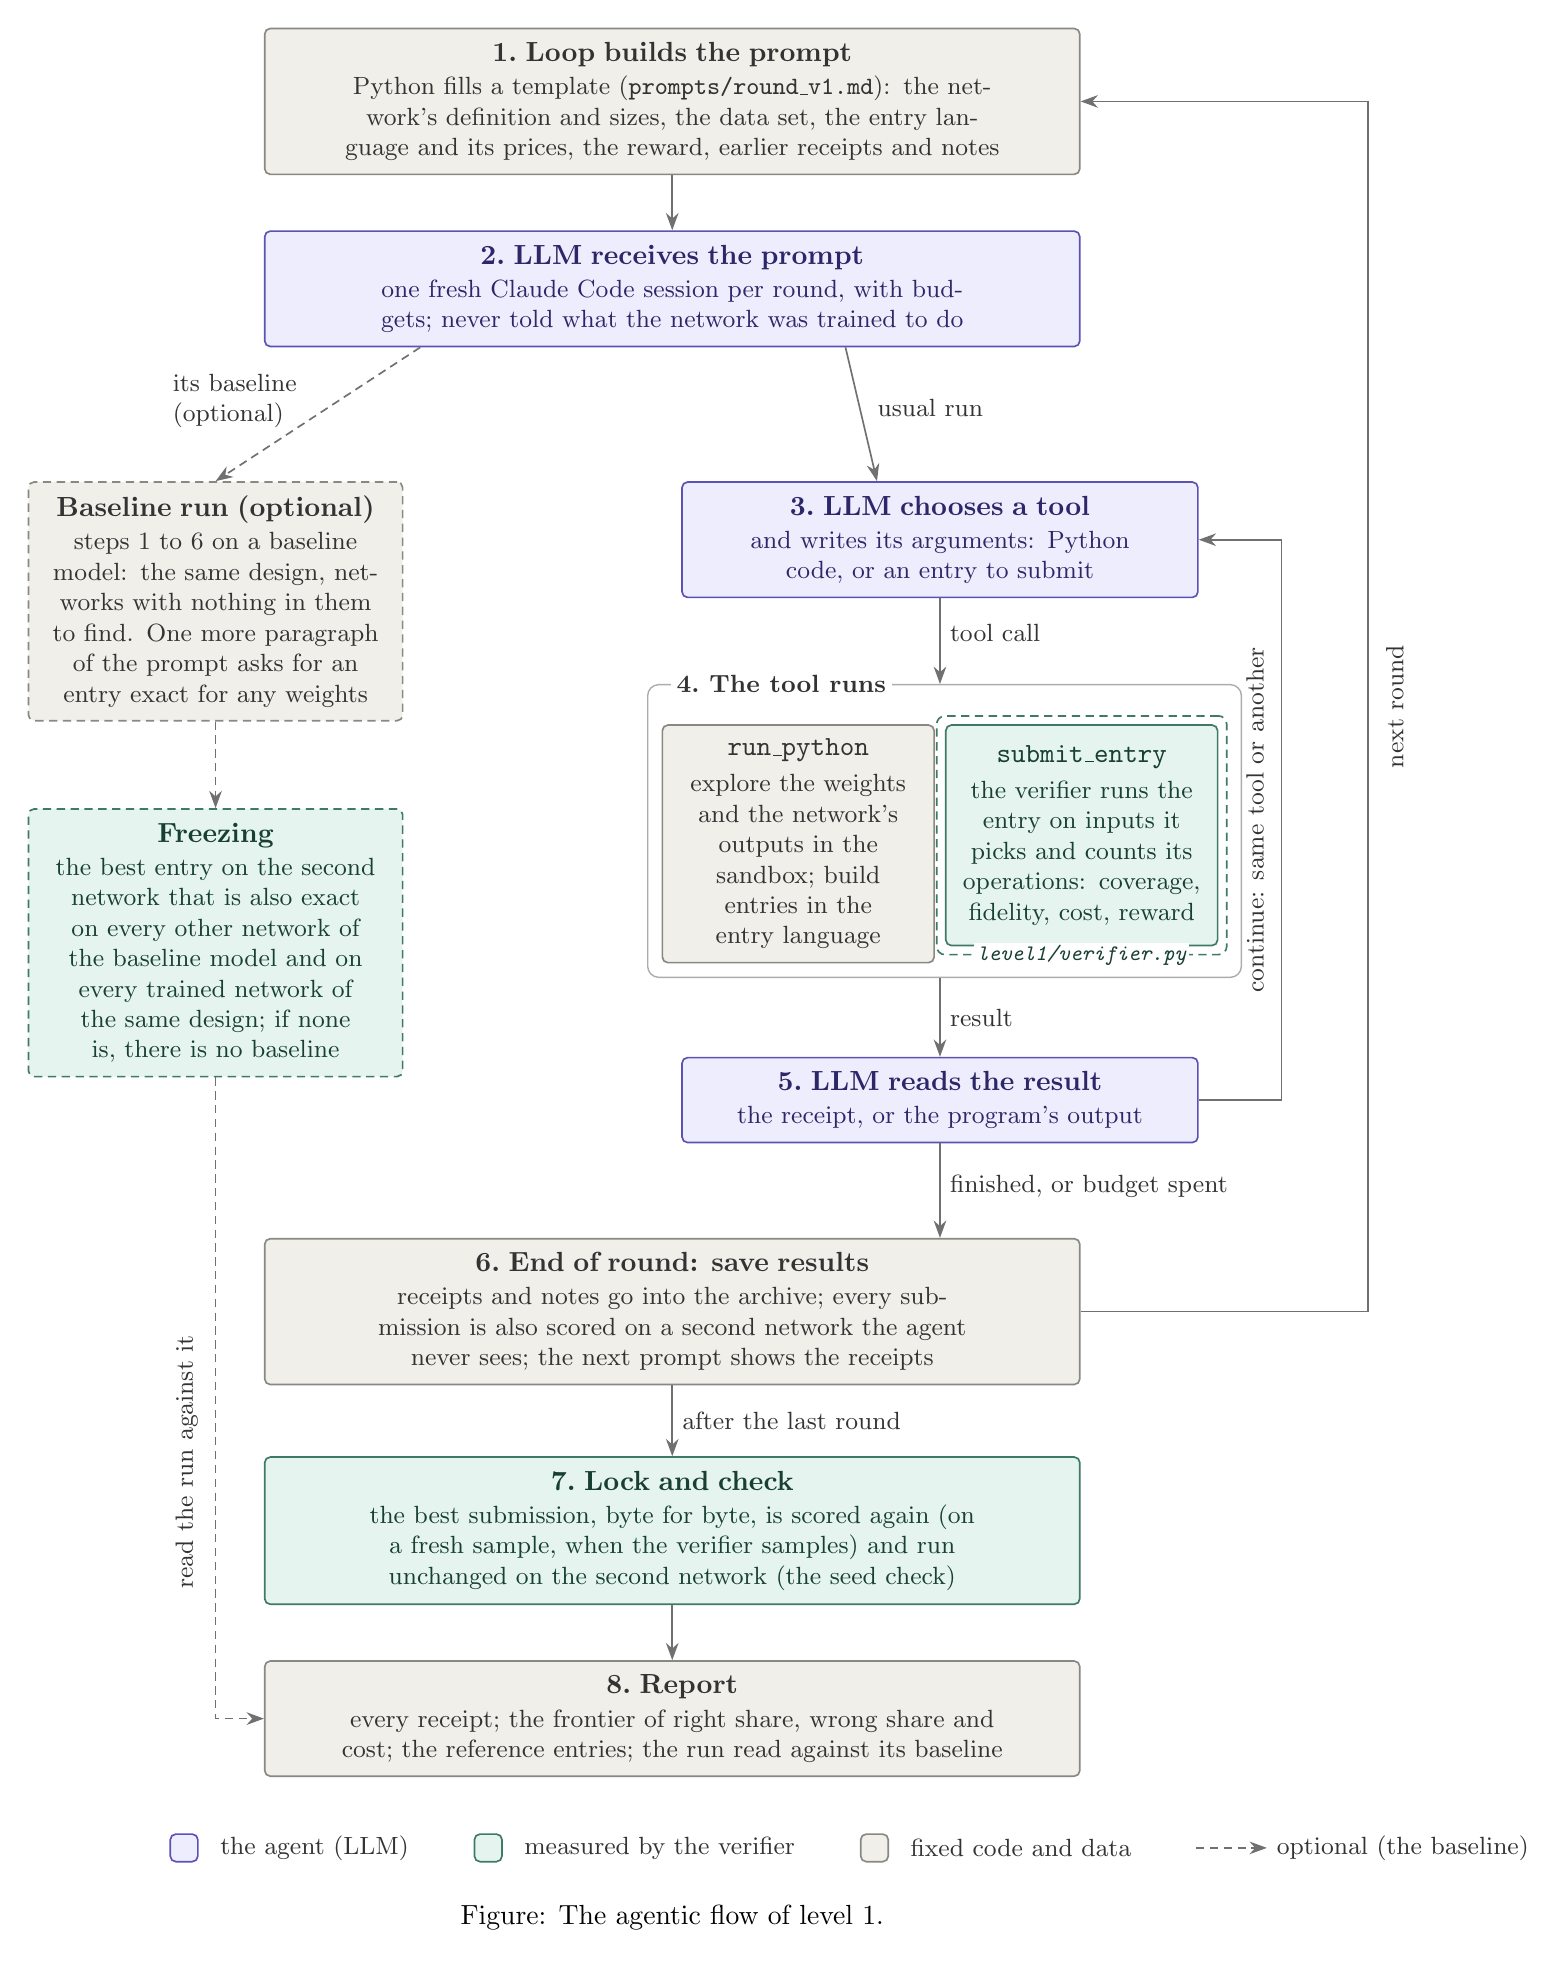
\begin{tikzpicture}

% 1, 2: the prompt, across the top
\node[fixed, text width=100mm] (p1) at (0,0) {\tit{1.\ Loop builds the prompt}
  Python fills a template (\texttt{prompts/round\_v1.md}): the network's definition and sizes,
  the data set, the entry language and its prices, the reward, earlier receipts and notes};
\node[agent, text width=100mm, below=7mm of p1] (p2) {\tit{2.\ LLM receives the prompt}
  one fresh Claude Code session per round, with budgets; never told what the network was trained to do};

% the usual run, on the right: steps 3 to 5
\coordinate (R) at (34mm,0);
\node[agent, text width=62mm, anchor=north] (p3) at ($(R |- p2.south)+(0,-17mm)$) {\tit{3.\ LLM chooses a tool}
  and writes its arguments: Python code, or an entry to submit};
\node[fixed, text width=31mm, minimum height=28mm, anchor=north] (py) at ($(p3.south)+(-18mm,-16mm)$) {\tool{run\_python}
  explore the weights and the network's outputs in the sandbox; build entries in the entry language};
\node[meas, text width=31mm, minimum height=28mm, anchor=north] (sub) at ($(p3.south)+(18mm,-16mm)$) {\tool{submit\_entry}
  the verifier runs the entry on inputs it picks and counts its operations: coverage, fidelity, cost, reward};
\begin{scope}[on background layer]
  \node[draw=measdraw, opt, rounded corners=3pt, line width=0.6pt, fit=(sub), inner sep=3pt] (ver) {};
  \node[draw=fixeddraw!70, rounded corners=4pt, line width=0.5pt, fit=(py)(sub)(ver), inner xsep=5pt, inner ysep=8pt,
        yshift=3pt] (tools) {};
\end{scope}
\node[fill=white, inner sep=2pt, font=\small\bfseries, text=fixedtext, anchor=west] at ($(tools.north west)+(3mm,0)$) {4.\ The tool runs};
\node[font=\footnotesize\itshape, text=meastext, fill=white, inner sep=1pt] at (ver.south) {\texttt{level1/verifier.py}};
\node[agent, text width=62mm, anchor=north] (p5) at ($(R |- tools.south)+(0,-10mm)$) {\tit{5.\ LLM reads the result}
  the receipt, or the program's output};

% its baseline, on the left, dashed
\coordinate (L) at (-58mm,0);
\node[fixed, opt, text width=44mm, anchor=north] (b1) at ($(L |- p2.south)+(0,-17mm)$) {\tit{Baseline run (optional)}
  steps 1 to 6 on a baseline model: the same design, networks with nothing in them to find. One more paragraph
  of the prompt asks for an entry exact for any weights};
\node[meas, opt, text width=44mm, below=11mm of b1] (b2) {\tit{Freezing}
  the best entry on the second network that is also exact on every other network of the baseline model
  and on every trained network of the same design; if none is, there is no baseline};

% 6, 7, 8: below, across
\node[fixed, text width=100mm, anchor=north] (p6) at ($(0,0 |- p5.south)+(0,-12mm)$) {\tit{6.\ End of round: save results}
  receipts and notes go into the archive; every submission is also scored on a second network the agent
  never sees; the next prompt shows the receipts};
\node[meas, text width=100mm, below=9mm of p6] (p7) {\tit{7.\ Lock and check}
  the best submission, byte for byte, is scored again (on a fresh sample, when the verifier samples)
  and run unchanged on the second network (the seed check)};
\node[fixed, text width=100mm, below=7mm of p7] (p8) {\tit{8.\ Report}
  every receipt; the frontier of right share, wrong share and cost; the reference entries;
  the run read against its baseline};

% arrows
\draw[arr] (p1) -- (p2);
\draw[arr] ($(p2.south)+(22mm,0)$) -- node[lab, right, pos=0.45, xshift=1mm] {usual run} ($(p3.north)+(-8mm,0)$);
\draw[arr, opt] ($(p2.south)+(-32mm,0)$) -- node[lab, left, pos=0.4, xshift=-4mm] {its baseline\\(optional)} (b1.north);
\draw[arr] (p3.south) -- node[lab, right, pos=0.4] {tool call} (p3.south |- tools.north);
\draw[arr] (p3.south |- tools.south) -- node[lab, right, pos=0.5] {result} (p5.north);
\coordinate (loop) at ($(tools.east)+(5mm,0)$);
\draw[arr] (p5.east) -| (loop |- p5.east) |- node[lab, pos=0.25, rotate=90, anchor=south, yshift=1mm] {continue: same tool or another} (p3.east);
\draw[arr] (p5.south) -- node[lab, right, pos=0.45] {finished, or budget spent} (p5.south |- p6.north);
\draw[arr, opt] (b1) -- (b2);
\draw[arr] (p6) -- node[lab, right, pos=0.5] {after the last round} (p7);
\draw[arr] (p7) -- (p8);
\draw[arr, opt] (b2.south) |- node[lab, pos=0.3, rotate=90, anchor=south, yshift=1mm] {read the run against it} (p8.west);
\coordinate (next) at ($(loop)+(11mm,0)$);
\draw[arr] (p6.east) -| (next |- p6.east) |- node[lab, pos=0.25, rotate=90, anchor=north, yshift=-1mm] {next round} (p1.east);

% legend and caption
\node[agent, minimum width=3.5mm, minimum height=3.5mm, inner sep=0pt] (l1) at ($(p8.south)+(-62mm,-9mm)$) {};
\node[lab, right=1.5mm of l1] (t1) {the agent (LLM)};
\node[meas, minimum width=3.5mm, minimum height=3.5mm, inner sep=0pt, right=7mm of t1] (l2) {};
\node[lab, right=1.5mm of l2] (t2) {measured by the verifier};
\node[fixed, minimum width=3.5mm, minimum height=3.5mm, inner sep=0pt, right=7mm of t2] (l3) {};
\node[lab, right=1.5mm of l3] (t3) {fixed code and data};
\draw[arr, opt] ($(t3.east)+(7mm,0)$) -- ++(9mm,0) node[lab, right] {optional (the baseline)};
\node[font=\normalsize, anchor=north] at ($(p8.south)+(0,-15mm)$) {Figure: The agentic flow of level 1.};
\end{tikzpicture}
\end{document}
